\documentclass[tikz,border=6pt]{standalone}
\usetikzlibrary{positioning,arrows.meta,fit,calc}
\begin{document}
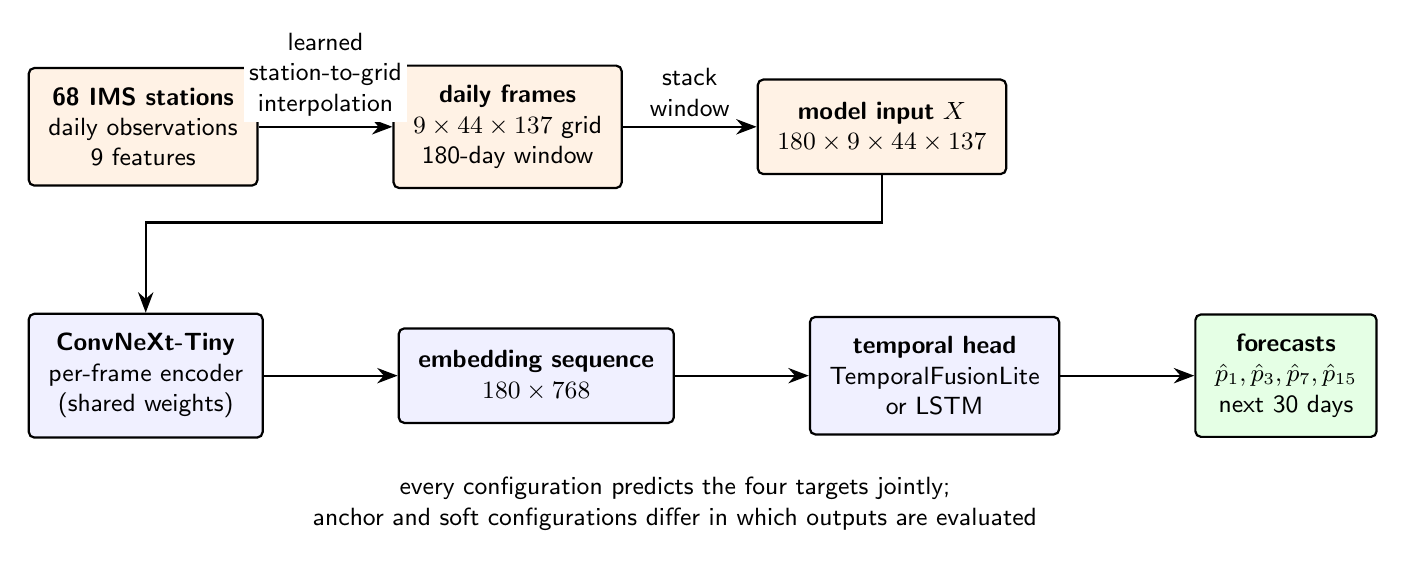
\begin{tikzpicture}[
  font=\sffamily\small,
  box/.style={draw, rounded corners=2pt, align=center, minimum height=12mm,
              inner sep=2.5mm, fill=blue!6, thick},
  data/.style={draw, rounded corners=2pt, align=center, minimum height=12mm,
               inner sep=2.5mm, fill=orange!10, thick},
  outp/.style={draw, rounded corners=2pt, align=center, minimum height=12mm,
              inner sep=2.5mm, fill=green!10, thick},
  arr/.style={-{Stealth[length=2.6mm]}, thick},
  lbl/.style={font=\sffamily\small, align=center, fill=white, inner sep=2pt},
  node distance=13mm and 17mm]

% ---- top row: data construction ----
\node[data] (stations) {\textbf{68 IMS stations}\\daily observations\\9 features};
\node[data, right=of stations] (frames) {\textbf{daily frames}\\$9\times44\times137$ grid\\180-day window};
\node[data, right=of frames] (sample) {\textbf{model input} $X$\\$180\times9\times44\times137$};

\draw[arr] (stations) -- node[lbl, above=0.5mm] {learned\\station-to-grid\\interpolation} (frames);
\draw[arr] (frames) -- node[lbl, above=0.5mm] {stack\\window} (sample);

% ---- bottom row: model ----
\node[box, below=16mm of stations.south west, anchor=north west] (encoder)
  {\textbf{ConvNeXt-Tiny}\\per-frame encoder\\(shared weights)};
\node[box, right=of encoder] (seq) {\textbf{embedding sequence}\\$180\times768$};
\node[box, right=of seq] (head) {\textbf{temporal head}\\TemporalFusionLite\\or LSTM};
\node[outp, right=of head] (y) {\textbf{forecasts}\\$\hat p_1,\hat p_3,\hat p_7,\hat p_{15}$\\next 30 days};

\draw[arr] (sample.south) -- ++(0,-6mm) -| (encoder.north);
\draw[arr] (encoder) -- (seq);
\draw[arr] (seq) -- (head);
\draw[arr] (head) -- (y);

% ---- variants note ----
\node[lbl, below=6mm of seq.south east, anchor=north, fill=none]
  {every configuration predicts the four targets jointly;\\anchor and soft configurations differ in which outputs are evaluated};
\end{tikzpicture}
\end{document}
